\documentclass[]{amsart}

\setlength\topmargin{-0.5in}
\setlength\headheight{15pt}
\setlength\headsep{15pt}
\setlength\footskip{25pt}
\setlength\textwidth{6.5in}
\setlength\oddsidemargin{0in}
\setlength\evensidemargin{0in}
\setlength\parindent{0.25in}
\setlength\parskip{0pt} % was 3pt
\setlength\textheight{9.0in}
\usepackage[fontsize=13pt]{scrextend}
\usepackage[margin=3cm]{geometry}% http://ctan.org/pkg/geometry
\usepackage{tabularx}% http://ctan.org/pkg/tabularx
\usepackage{booktabs}% http://ctan.org/pkg/booktabs
\newcolumntype{Y}{>{\raggedleft\arraybackslash}X}% raggedleft column X
\usepackage{amssymb,latexsym,amsmath}
\usepackage{graphicx,xcolor}
\usepackage[round]{natbib}
\usepackage{booktabs}
\usepackage{multirow}
\usepackage{pdflscape}
\usepackage{datetime}
\usepackage{afterpage}
\usepackage{graphicx}
\usepackage{dcolumn}
\usepackage{lscape}
\usepackage{pdfpages}
\usepackage[justification=centering]{caption}
\usepackage[toc,page]{appendix}
\usepackage{afterpage}
\setcounter{MaxMatrixCols}{10}
\providecommand{\jel}[1]{{{JEL classification:}} #1}
\providecommand{\keywords}[1]{{{Key words:}} #1}
\pagestyle{plain}


\title{Electricity Intensity Forecast: A Time Series Model of Convergance Approach}
\author{Lior Gallo \\
The Bank of Israel \\
The Hebrew University of Jerusalem \\
This Version: \today \\
\textit{First draft. Please, give me feedback and do not quote or circulate. }}

\begin{document}
\maketitle
	\begin{abstract}
	This paper reports the results of a long term forecast of electricity intensity for the OECD countries. Following the observation that electricity intensity in the OECD countries converges, I estimate a set of nine time series models and choose the best preforming three to produce forecast. Using each of the three models this paper presents forecast for total electricity intensity, households' electricity intensity and the electricity intensity of the major economic sectors in each OECD country. Average electricity intensity in the OECD according to the forecast will decrease in the next ten years at a rate  of 1.5 - 2.8 percent per year.
	\end{abstract}

\newpage

\tableofcontents

\newpage

\section{Introduction}

This paper utilities the observation that electricity intensity converges over time to construct a long term forecast of electricity intensity for the OECD counties.\footnote{Electricity intensity is defined as the ratio between electricity and GDP.} To forecast electricity intensity I estimate a set of nine time-series models that are built on the intuition of \cite{barro1992convergence}'s $\beta-convergence$ test. I examine the in-sample and out-of-sample performances of the models and choose the best four, from which I calculate electricity intensity forecast. For each OECD country the paper reports electricity intensity forecast for the total economy, for the households' and for each of the five economic branches that comprise the GDP of these countries, namely: Agriculture, mining and querying, manufacturing, commercial services, construction. To validate that electricity intensity indeed converges the paper estimate and reports the results of the two well known convergence tests, namely: \cite{barro1992convergence}'s $\beta-convergence$ test and \cite{PhillipsSul2007}'s $\sigma-convergence$ test. 

\bigskip

Table 1 illustrates the central results of the paper. The table shows the average change of electricity intensity in the OECD countries. The first raw presents actual change in intensity while the remaining three rows present the forecast according to the best preforming models. The first, the second and the third columns presents past growth rates of electricity intensity. These columns reveal that average electricity intensity in the OECD countries decreased in the past. In addition it reveals that the pace of decrease accelerate. During the 90's average electricity intensity decreased at an annual rate of ($-0.63$) percent. Later in the first decade of the 21 century the decrease accelerated to an annual rate ($-0.77$). Acceleration hasn't stop there and in the last five years electricity intensity decreased at an annual rate of ($-1.21$). It is easy to see that the models manage to imitate the past decrease in intensity, the magnitude of the decrease as well as the acceleration. The fourth and fifth columns present the central result of the paper which is the models' future forecast. These forecast manifest both the decrease of electricity intensity as well as the acceleration of the decrease. Whereas all models forecast a decrease each estimate different rate of acceleration. 

    
\begin{table}[htb] \centering
  \caption{Electricity Intensity in the OECD Countries: Past and Future}
   \label{tbl:Central_Results}
			\resizebox{0.9\textwidth}{!}{
\begin{tabular}{lccc|cc}
\hline
& \multicolumn{3}{c}{Past Averages} & \multicolumn{2}{c}{Future Averages} \\ 
\cline{2-6} \\
Model & 1992-1999 & 2000-2009 & 2010-2015 & 2016-2025 & 2026-2035 \\ 
\hline
\hline
Real  & $-0.63$ & $-0.77$ & $-1.21$ &  &  \\
Model 1  & $-0.47$ & $-0.83$ & $-1.17$ & $-1.50$ & $-1.93$ \\
Model 2  & $-0.53$ & $-0.80$ & $-1.26$ & $-2.18$ & $-4.67$ \\
Model 3 & $-0.42$ & $-0.81$ & $-1.60$ & $-2.78$ & $-4.63$ \\
\hline 
\multicolumn{6}{l}{\begin{footnotesize}Electricity intensity is defined as the ration of electricity and GDP.\end{footnotesize}} \\
\multicolumn{6}{l}{\begin{footnotesize}Model 1 is a reduced form of \cite{barro1992convergence} as shown in equation (\ref{RF_full}).\end{footnotesize}} \\
\multicolumn{6}{l}{\begin{footnotesize}Model 2 is a genralization of \cite{barro1992convergence} as shown in equation (\ref{BSM_full}).\end{footnotesize}} \\
\multicolumn{6}{l}{\begin{footnotesize}Model 3 is a generalization of and AR(1)  as shown in equation (\ref{dif_ar_full}).\end{footnotesize}} \\
\hline
\end{tabular}
}
		\end{table} 

\bigskip

The long-term decrease in electricity intensity has been observed and documented in many papers in the past and it is manifested in Figure 1.\footnote{See : World Energy Outlook 2016, 2018} The figure portraits GDP-PC and electricity intensity in the OECD countries through the years. For means of visualization the figure also include trend lines to the observation of each country. The figure reveals a clear negative correlation between electricity intensity and development. Countries with high level of development use less electricity for the production of each unit of GDP. The negative correlation between development and electricity intensity is also manifested an the country level where each country's development trough the years is associated with decrease in electricity intensity. It is worth noting that although the global trend is obvious and can be illustrated with a simple graph, eight states differ from the common trend: Portugal, Italy, Greece, Spain, Mexico, Chile, Turkey and Republic of Korea. The reasons for the increase in their intensity are beyond the scope of this paper although from first glance it looks as if they simply converge to the global trend from below.\footnote{Appendix XXX elaborate on these countries and especially on Korea which act differently.}

\begin{figure}[h]
    \centering
\caption{Electricity Intensity and GDP per capita Trends in the OECD Countries}
    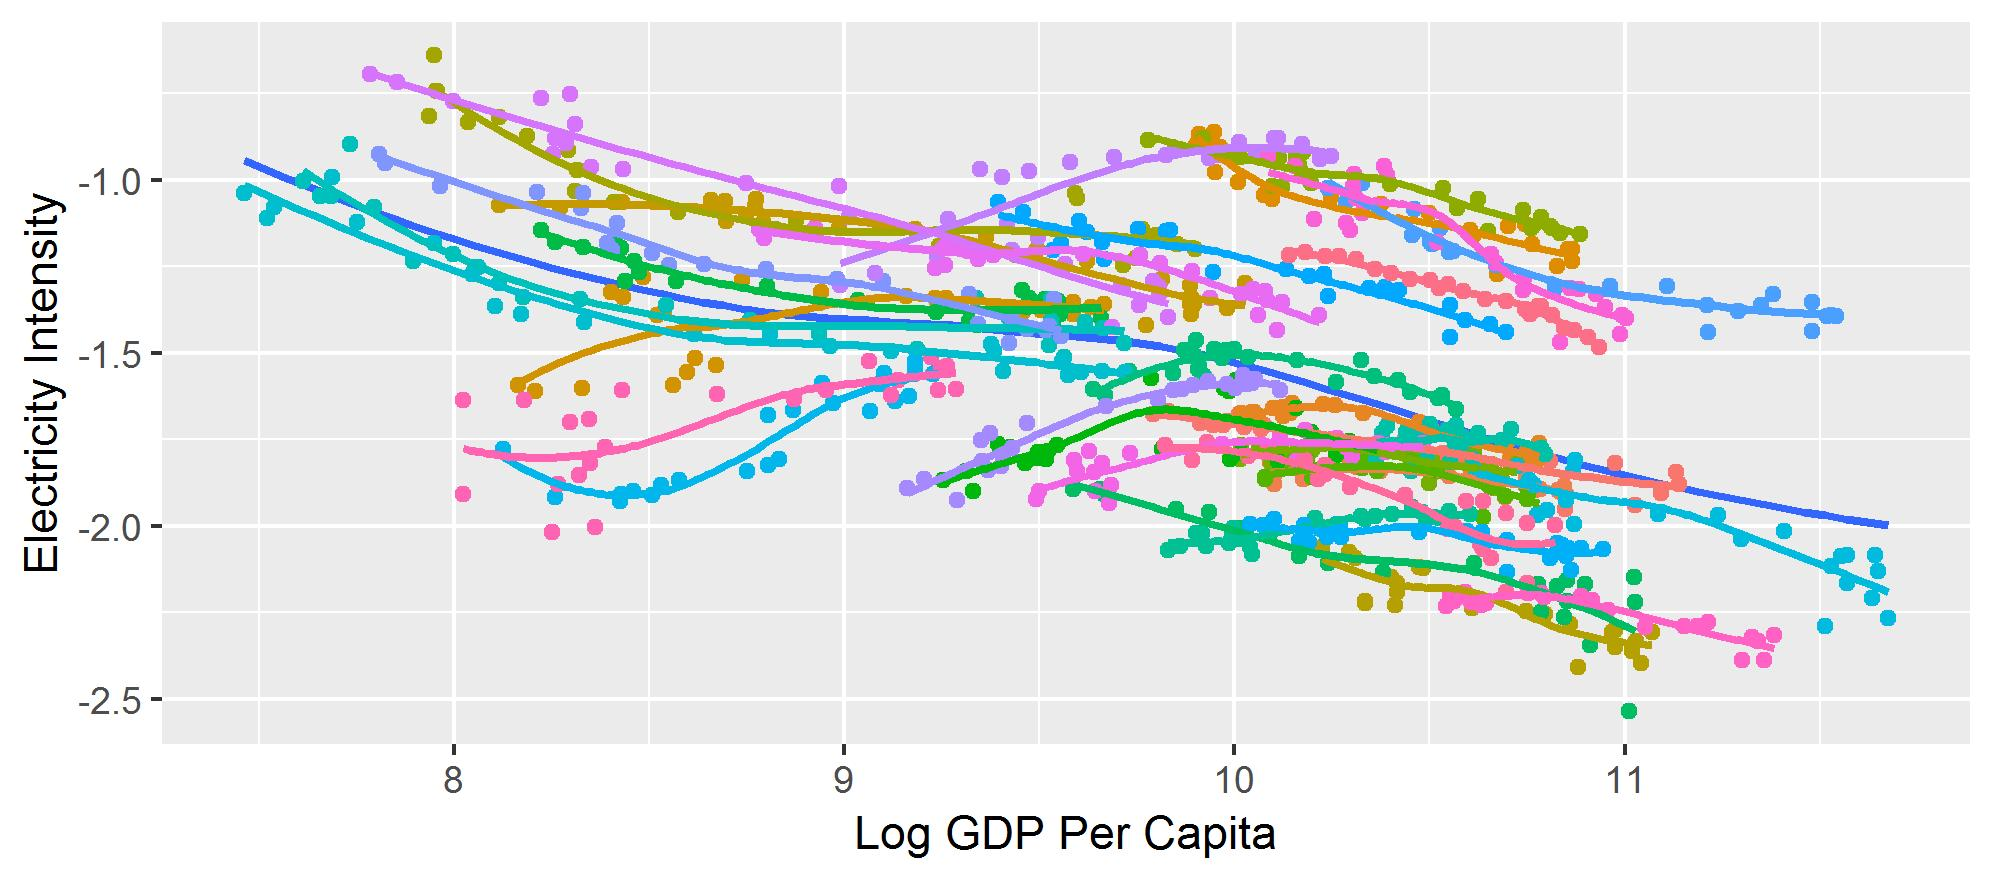
\includegraphics[width=1\textwidth]    {Electricity_Intensity_GDPPC}
    \label{Fig_intro}
\end{figure}

\bigskip

The importance of constructing a forecast of electricity demand stems primarily from the implication to policy design. All around the world government agencies regulate electricity markets in general, and the supply of electricity in particular. The supply of electricity depends on investments that takes place long before the supply of the first unit of electricity meets the demand. Hence, an accurate forecast of electricity demand enables efficient design in planning of future supply and facilitates the investment decision. An efficient design would guarantee minimization of the gaps between supply and demand for electricity where access demand might erect costs due to the value of lost load and access supply (mostly) due to the opportunity costs of capital.\footnote{Other reasons that relate to access supply are lost due to long term fuel contracts that often include a take or pay mechanism or reason that are related to the design of market structure. For example it might aggravate the market failure of first entrant and hence cause long term social cost.}

\bigskip

Electricity demand forecasts are also one of the central inputs of environmental policy designers. Environmental policy targets such as reduction of green house gases or improvement of energy efficiency are often built relative to some basic scenario. An ex-ante forecast of electricity intensity provides such scenario and hence it is a crucial building block for policy designers. This issue become even more meaningful given the fact that the world is electrifying - electricity share in total energy consumption increases in the last several decade.

\bigskip

In addition to the forecasts electricity intensity of the total economy the paper reports the forecast of electricity intensity of households and of each of the five economic branches that comprise the GDP, namely: Agriculture, mining and querying, manufacturing, commercial services, construction. Sectoral electricity intensity forecasts are important from both the energy and environmental policy perspective. Energy researches have long realized the importance the decomposition of energy demand to the industrial sectoral mix and the development of each sector's energy intensity. Although the research on this issue started in the late 70's, it was institutionalized by the extensive work of \cite{ang1987structural,ang1995decomposition,Ang1999,ang2004decomposition}.

\bigskip

Sectoral electricity intensity forecasts are important to energy regulators due to the fact that different sectors or more broadly different types of consumers exhibit different demand schemes. For example the hourly demand curve of the manufacturing sector is often flatter then the hourly demand of the services sector or that of the households who exhibit similar demand scheme with major picks in the early evening. Different demand curves require different supply technologies for example technologies that are better coping with long term supply and those who are better coping with picks. Hence, forecasts of different types of consumers is a critical input in the design of electricity policy and the investment decision. In terms of environmental design sectoral forecast are important because many environmental regulation are determined on a sectoral basis. Sectoral intensity analysis enables to identify sectoral bottle necks and design appropriate energy efficiency policies. 

\bigskip

As mentioned above the central theme of the forecast in this paper is the notion of the long term convergence patter of electricity intensity. To explore this notion the paper draws on two well known convergence models. The convergence of intensity describe a situation in which the dispersion of electricity intensity of different countries decrease over time. To the extent that this type of convergence relates to the variance of intensity over time it is called: $\sigma-convergence$. A different way to think about convergence is a situation in which growth rates of those countries with low level of intensity tend to be higher then those with high levels of intensity. In addition these high growth rates tend to decrease as electricity intensity increases over time. This type of convergence reflects in data when initial levels of intensity are negatively correlated to intensity growth rates. To the extend that this type of convergence can be estimated using a simple regression model it was named: $\beta-convergence$. 

\bigskip

This intuition was formulated into formal statistical models in the economic growth literature to test for convergence of development between countries. The first model is from the seminal papers of \cite{barro1992convergence} and \cite{sala1996classical} who developed a test for the $\beta-convergence$. The model regresses average intensity growth rates on initial level of intensity. A negative correlation between initial levels and average growth rates indicates convergence. In the current paper I report the results of the convergence test of \cite{barro1992convergence} as well as the results of a reduced form of their model. I find that the reduced form model better fits for the purpose of forecasting relative to the original specification of \cite{barro1992convergence} which was build specifically for statistical inference.

\bigskip

The second model is from \cite{PhillipsSul2007} who developed a semi-parametric statistical test that examine the hypothesis that the variance decreases over time. i.e., a test for the $\sigma-convergence$. Their method boils down to estimation of a regression model in which the variance of intensity between countries is a negative-non-linear function of time. Just like in the case of \cite{barro1992convergence} the model of \cite{PhillipsSul2007} fits the purpose of testing for convergence however not necessary for the purpose of forecasting. In the current paper I use this model to examine if sigma convergence can be found in the data and compare this result with those of the other models.

\bigskip

As mentioned above the convergence of electricity intensity is a well known fact. The intensity convergence has been documented in many papers in the energy economic literature. However, while the vast literature on the convergence focus on (primary) energy intensity the literature on electricity intensity is narrower.\footnote{Notable papers of energy convergence are: \cite{MulderGroot2012}, \cite{MohammadiRam2017}, \cite{ApergisChristou2016}, \cite{BurnettMadariaga2017}, \cite{Fallahi2017} \cite{AdhikariChen2014}. For a recent symposium on this subject see: \cite{ApergisEwingPayne2017}}

\bigskip

Several papers examined the question of convergence of electricity intensity in the past and the motivation for the current paper relay on their results. Nevertheless, the current paper differs from past work on this subject by comparing the results of these models. In addition the paper presents the results of electricity intensity convergence both at the country level and at the sector level and with both tests, namely \cite{barro1992convergence} and \cite{PhillipsSul2007}.

\bigskip

Early papers on this subject used basic econometric methods and visualization to test for convergence. \cite{MazaVillaverde2008} use data from 98 countries between 1980 and 2007 to examine whether there is a $\beta-convergence$ of household's per capita electricity consumption. Using an integrated autoregressive model their estimation support the existence of convergence. In addition, using non-parametric methods, they showed that the convergence process is relatively slow. In their paper they present visual illustration that the variance decreases over time however without a statistical test to measure it. In the current paper I present results of statistical convergence test using several methods and produce forecasts for electricity from them. \cite{Liddle2009} also present visual illustration that the variance decreases over time. In addition \cite{Liddle2009} presented estimation of linear time trend to tests for the convergence of electricity consumption in the IEA / OECD countries between 1971 and 2005.

\bigskip

Following \cite{MiketaMulder2005}'s specification \cite{MohammadiRam2012} estimated $\beta-convergance$ equations of electricity using a reduced form of \cite{sala1996classical}. The authors used a sample of 108 countries between 1971 and 2007 and their results from a quantile regression concluded that while there is convergence in electricity consumption, it is slow. In the current paper I present results that are build on a model similar to their reduced form as well as from the specification of other models. 

\bigskip

In a more recent paper \cite{Kim2015} examined the convergence of electricity intensity using data from 109 countries between 1970 and 2009. \cite{Kim2015} estimated \cite{PhillipsSul2007}'s $\sigma$ convergence tests for all countries in the database and another test for developed countries. The results are that among the developed countries there are groups that converge to the same intensity. This phenomenon is known in the literature as club convergence. As mentioned above \cite{PhillipsSul2007}'s semi-parametric convergence test dose not allow to estimate forecasts. In relation to \cite{Kim2015}'s work the current work elaborate on \cite{PhillipsSul2007}'s work and develop a structural-model that fit for forecast.

\bigskip

\cite{LeChangPark2017} examine the convergence of per capita energy and electricity per capita in the APEC countries using annual data between 1989 and 2012. They use Unit Chart and Sequential Panel Selection Model. When using Unit CHART, their results indicate convergence in all countries. The use of SPSM indicates convergence in 15 of the 19 countries for energy and 17 out of 19 for electricity. This article is cute and interesting in particular because of the method they present that I do not know. Also since it was recently published in EE then it will be able to give you direction where to aim.

\bigskip

The evidence on electricity intensity convergence are not limited to westeran countries alone. Using several convergence tests \cite{HerreriasLiu2013} found  electricity intensity convergence Chinese provinces.\footnote{They presented test from: \cite{lee2003minimum}, \cite{kapetanios2003testing}, \cite{PhillipsSul2007} and \cite{hansen2000sample}.} They identify three clubs to which to provinces converge. XX Papers on states in the USA. Paper on easteren countris. Finish the surveyXXXX

\bigskip

The paper adds to the literature by reporting a simple, transparent and objective forecast of electricity demand. To this end the analysis uses the most prevalent methods in the field and freely available data base. This feature of the analysis is of a great importance for policy designers who wish to reproduce the results and adjust the models to their use.\footnote{For the R codes of the paper and a short guide of who to reproduce the results see: http:XXX.} The rest of the paper is constructed as follows. The next section surveys the literature on convergence of energy intensity. The third section formalize the analytical framework. The fourth section reports the data and the results and the final section concludes.

\bigskip

\section{Analytical Framework: From Convergence-test models to time-series models for forecasting}

\bigskip

The objective of the analysis is to study the dynamic behaviour of electricity intensity concentrating on the notion of convergence. For this purpose the section formulates a set of econometric tests that are used in the literature to examine the convergence hypothesis. Some tests are build on specifications that enable to produce forecast with no cost while others require some adjustment. The set of models is comprised of two groups. Each of which stems from one of the two models that are currently serve as the working-horses in the economic literature to test for convergence, namely the models of \cite{barro1992convergence} and \cite{PhillipsSul2007}. The econometric literature suggests plenty of other models to test and examine the notion of convergence, each uses different specification to deal with different econometric challenges.\footnote{For example: \cite{lee2003minimum}, \cite{kapetanios2003testing}, and \cite{hansen2000sample}.} Nevertheless, the models of \cite{barro1992convergence} and \cite{PhillipsSul2007} still remain the working horses of the filed. 

\bigskip

Each one of the econometric groups in the set includes the original specification of the convergence test as well as several reduced form versions of this model. 
Comparing the estimation results of the original specification with the results of the reduced form version pure some light on the importance of the econometric challenges with which the models attempt to cope. Notably, the initial motivation to develop the models of \cite{barro1992convergence} and \cite{PhillipsSul2007} stems from the fact that the data do not necessarily obeys the assumptions on which the classical models are built such as stationarity, co-integration, balanced panels, etcetera. Furthermore, in addition to illustrating the magnitude of the bias with which the special models cope, I find that in many cases the reduced form models preform better then the original specifications in terms of forecasting. Indeed, this is not a surprising result simply because the convergence tests were build for the purpose of statistical inference and not necessarily for the purpose of forecasting.

\bigskip

To rank the performances of each model I use standard in-sample and out-of-sample measures. The in sample measures include adjusted R square and mean square error. For the out of sample measure I use the special panel data structure to construct a simple bootstrap out of sample mean square error. This is done by estimating the model on a random sample of the countries and calculating the mean square error on the rest of the countries. I repeat this process 30 times and calculate the average mean square error of these 30 simulations. Before we dive into the formulation it is important to note that the exposition through the section relay heavily on those of \cite{barro1992convergence} and \cite{PhillipsSul2007} as well as that of \cite{sala1996classical}, \cite{durlauf2005growth} and \cite{young2008sigma}.

\bigskip

Define the electricity intensity of country $j$ in sector $k$ at time $t$ as the ratio of electricity $(E)$ use of this sector and the gross domestic product $(GDP)$ of that sector: 

\begin{equation}
I_{j,k,t} \equiv \frac{E_{j,k,t}}{GDP_{j,k,t}}
 \label{Intensity} 
\end{equation}

\bigskip

To ease the notation I abstract for now from sectors and will return to it when it is relevant. 

\bigskip

\subsection{The $\beta-test$}

The first group of models to test and estimate convergence rate is called the $\beta-convergance$. These tests are build on a regression in which the dependent variable is the rates of change in the intensity of the electricity, and the independent variable is the intensity of electricity in the base year. If intensity converges, the coefficient of intensity in the base year will be negative, i.e., the higher the intensity of the electricity intensity in the base year the slower the rate of change of intensity, so that in the long term the levels (or change rates) converge. In order to test for convergence \cite{barro1992convergence} suggested a following specification:

\bigskip

\begin{equation}
\frac{i_{j,t}-i_{j,t0}}{t-t_0}  = \alpha_{BSM} - \left( \frac{1- e^{-\beta_{BSM}(t-t_0)}}{t-t_0} \right) i_{j,t_0}+u_{i, t}
\label{BSM_original}
\end{equation}

\bigskip

where $i_{j,t} \equiv log(I_{j,t})$, $u_{i,t}$ is assumed to be white noise, $i_{j,t_0}$ is the intensity in the base year $t_0$. When $(\beta_{BSM} \geq 0)$ equation (\ref{BSM_original}) estimates the average change rate of intensity as a constant term ($\alpha_{BSM}$) which is offset by second therm on the right hand side of the equation. When $(\beta_{BSM} \geq 0)$  the effect of the second term diminishes with time.  To see this not that:
$\left( \frac{1- e^{-\beta_{BSM}(t-t_0)}}{t-t_0} \right) \xrightarrow{t-t_0 \rightarrow \infty} 0$. Hence, ($\alpha_{BSM}$) here can be interpreted as the average change rate in the long run. As \cite{sala1996classical} explains the main advantage of the model in (\ref{BSM_original}) relative to a simple time-series model is that (\ref{BSM_original}) overcomes a bias that might be caused due to different time length.\footnote{Another advantage is that the formulation in (\ref{BSM_original}) intimately relate to the economic growth model for which it was build. To the extent that the current work dose not deal with the economic growth issue the relevant advantage is the first. For thorough explanation of these advantages see \cite{barro1992convergence} and \cite{sala1996classical} or \cite{durlauf2005growth}} To illustrate this point and understand the specification equation (\ref{ar_original}) formulates the log of the intensity as an AR(1) stochastic process:

\begin{equation}
i_{j,t} = \alpha_{AR} + (1-\beta_{AR})i_{j,t-1}+u_{i,t}
 \label{ar_original} 
\end{equation}

The auto-regressive process in (\ref{ar_original}) converges as long as $ 0 \leq \beta_{AR} \leq 1$ hence the term $\beta-convergance$. Substructure $i_{j,t-1}$ from both sides of (\ref{ar_original}) sums up to:

\begin{equation}
\Delta i_{j,t} = \alpha_{AR}-\beta_{AR} i_{j,t-1}+u_{i,t}
\label{dif_ar_original}
\end{equation}

where $\forall Z: \Delta z_{i,t} \equiv z_{i,t}-z_{i,t-1}$. To understand the link between (\ref{dif_ar_original}) and (\ref{BSM_original}) it is instructive to write the AR(1) process in (\ref{ar_original}) as a function of the intensity at $t_0$:

\begin{equation}
i_{j,t} = \alpha_{AR}\sum_{\tau = 0}^{t-t_0-1}(1-\beta_{AR})^{\tau}+(1-\beta_{AR})^{t-t_0}i_{j,t_0}+\sum_{\tau=1}^{t-t_0} (1-\beta_{AR})^{t-t_0-\tau}u_{i,t+\tau}
\label{AR_adj1}
\end{equation}

Substructing $i_{j,t_0}$ from both sides and dividing by $t-t_0$ yields the following equation:

\begin{equation}
\frac{i_{j,t}-i_{j,t_0}}{t-t_0} = \alpha_{AR}\frac{\sum_{\tau = 0}^{t-t_0-1}(1-\beta_{AR})^{\tau}}{t-t_0}-\frac{(1-(1-\beta_{AR})^{t-t_0})}{t-t_0}i_{j,t_0}+\frac{\sum_{\tau=1}^{t-t_0} (1-\beta_{AR})^{t-t_0-\tau}u_{i,t+\tau}}{t-t_0}
\label{AR_adj2}
\end{equation}

\bigskip

Let us start by comparing the expressions that proceed the initial intensity ($i_{j,t_0}$) of both (\ref{BSM_original}) and (\ref{AR_adj2}). The analysis here assumes that the models indeed converge that is : $(\beta_{BSM} \geq 0)$ and  ($0 \leq \beta_{AR} \leq 1$). First, note that both expressions converge to zero as time goes to infinity. In that manner both models impose such formulation to the data that the average change rate of the series shrinks over time. However, while the average change of the model in (\ref{BSM_original}) converge to ($\alpha_{BSM}$), the average change of the model in (\ref{AR_adj2}) converges to zero. To see this note that:
$$\alpha_{AR}\frac{\sum_{\tau = 0}^{t-t_0-1}(1-\beta_{AR})^{\tau}}{t-t_0} \ \xrightarrow{t-t_0 \rightarrow \infty} 0  \Leftrightarrow E(i_{j,t})=\frac{\alpha_{AR}}{1-\beta_{AR}}$$ Hence, in the AR(1) model the level of intensity converge to a constant which is the same as saying that the average change converges to zero. On the other side of the limit both expressions converge to $\beta$ as time goes to zero. To see this note that:
\begin{equation}
\frac{\partial (1-(1-\beta_{AR})^{t-t_0})}{\partial {(t-t_0})} = -ln(1-\beta_{AR})\cdot(1-\beta_{AR})^{t-t_0} \xrightarrow{t-t_0 \rightarrow 0} -ln(1-\beta_{AR}) \sim \beta_{AR}
\label{d_lag}
\end{equation}

\begin{equation}
\frac{\partial (1- e^{-\beta_{BSM}(t-t_0)})}{\partial {(t-t_0})} = \beta_{BSM} e^{-\beta_{BSM}(t-t_0)} \xrightarrow{t-t_0 \rightarrow 0} \beta_{BSM} 
\label{d_exp}
\end{equation}

The analysis above illustrates the differences and the resemblance between the models. In both models the average change decrease over time and converge to the steady state change. The AR(1) model assumes that change in intensity converges to zero while the one in (\ref{BSM_original}) assumes convergence to a rate of ($\alpha_{BSM}$).  

\bigskip

The third model with which I analyze the data is a reduced form version of (\ref{BSM_original}):

\begin{equation}
\frac{i_{j,t}-i_{j,t0}}{t-t_0}  = \alpha_{RF} +\beta_{RF} i_{j,t_0}+u_{i, t}
\label{RF_original}
\end{equation}

This model enables to estimate the average change in intensity as a constant plus some initial year specific effect. Note that in this model neither intensity nor the intensity change converges between counties over time. When ($\beta_{RF} \leq 0 $) this model fits the notion of temporary convergence. The model in (\ref{RF_original}) fits constant average change to each country. If ($\beta_{RF} \leq 0 $) countries with low intensity will experience a higher intensity growth. However, here the growth dose not decreases as their intensity changes but rather remains constant. Hence, after the convergence in intensity they will continue to grow fast which will cause divergence in intensity. To the extent that ex-ante we should not drop this possibility I estimate this model as well.

\bigskip

In the next section I present the estimation results of a generalized version of the three model above. Here I present these generalization as well as the interpretation of their possible results. The first model is a generalization of the AR(1) model. I elaborate on the interpretation of this model while the intuition follows the same line of thought.

\bigskip

\begin{equation}
\Delta i_{j,t} = \alpha_{AR}+ \beta_{AR} i_{j,t-1}+\gamma_{AR} t+\delta_{AR} i_{j,t-1}t+u_{j,t}
\label{dif_ar_full}
\end{equation}

\bigskip

The generalization examine the possibility of time trend and in addition that the lag variable coefficient depends on time. This is a non-stationary model with time trend and decreasing marginal effect of the initial year on initial value. To see this note that the expectation of this model is:

\bigskip

\begin{eqnarray}
E (i_{j,t}) & = & \frac{\alpha_{AR} + \gamma_{AR} t}{1 - \beta_{AR} - \delta_{AR}t}
\end{eqnarray}

\bigskip
 
Under the following assumptions the generalized model can be adjusted and interpreted as follows:

\bigskip

$(A): \  0 \leq \beta_{AR} \leq 1, \ \gamma_{AR} = 0, \ \delta_{AR} = 0  \ \  $

\bigskip

Model (A) is the simple AR(1) model that was presented in (\ref{ar_original}). To the extent that this is a stationary model its expectation is constant: $E (i_{j,t}) =  \frac{\alpha_{AR}}{1 - \beta_{AR} }$.

\bigskip
 
$(B): \  0 \leq \beta_{AR} \leq 1, \ \gamma_{AR} \neq 0, \ \delta_{AR} = 0  \ \  $

\bigskip

Model (B) is a non-stationary model of AR(1) with trend or otherwise an ARIMA(1,1,0). The expectation of this model changes with time at a rate of: $\frac{\gamma_{AR}}{1 - \beta_{AR}}$ which means that the sing of $\gamma_{AR}$ determines the direction of the trend. 

\bigskip

$(C): \ 0 \leq \beta_{AR} \leq 1, \ \gamma_{AR} \neq 0, \ \delta_{AR} \neq 0  \ \  $

\bigskip

Under this specification the lag coefficient is $(\beta_{AR}+\delta_{AR} t)$ which allows for the correlation between initial year and current growth to change with time. As time goes to infinity the long term expectation of this model converges to the constant $-\frac{\gamma_{AR}}{\delta_{AR}}$. To be more concrete this model enables to test each one of the following assumptions as well as their linear combinations: 

\bigskip

$H_0: \gamma_{AR} \neq 0 \leftrightarrow $   Data has time trend.

$H_0: \delta_{AR} \neq 0 \leftrightarrow $  Converges rate changes with time.

\bigskip

The second model is a generalization of \ref{BSM_original}:

\bigskip

\begin{equation}
\frac{i_{j,t}-i_{j,t0}}{t-t_0}  = \alpha_{BSM} - \left( \frac{1- e^{-\beta_{BSM}(t-t_0)}}{t-t_0} \right) i_{j,t_0}+ \gamma_{BSM}(t-t_0)+ \delta_{BSM}i_{j,t_0}(t-t_0)+u_{i, t}
\label{BSM_full}
\end{equation}

\bigskip

The interpretation of these test is different:

$H_0: \gamma_{BSM} \neq 0 \leftrightarrow $   Long term change is not constant but changes with time.

$H_0: \delta_{BSM} \neq 0 \leftrightarrow $  Converges rate changes with time in addition to the change imposed by the functional form.

\bigskip

Finally I dis-entrhrol from the functional form in (\ref{BSM_original}) and present a reduced form version of \cite{barro1992convergence} which enables to test some of these assumptions.

\bigskip

\begin{equation}
\frac{i_{j,t}-i_{j,t0}}{t-t_0}  = \alpha_{RF} +\beta_{RF} i_{j,t_0}+\gamma_{RF} (t-t_0) +\delta_{RF} i_{j,t_0}(t-t_0)+u_{i, t}
\label{RF_full}
\end{equation}

$H_0: \gamma_{BSM} \neq 0 \leftrightarrow $   Long term change is not constant but changes with time.

$H_0: \delta_{BSM} \neq 0 \leftrightarrow $  Initial intensity effect changes with time in addition.

\bigskip

\subsection{The $\sigma$-test}

The second approach to test for convergence relies on the intuition that the dispersion between countries decreases over time. To the extent that these models estimate the dynamics of the variance of intensity and not the intensity process itself it is not possible to use them for forecasting but only for testing for convergence. The next section develop a model that is build on the intuition of these models and enables forecasting. It is worth mentioning at this point the relationship between the $\beta-convergence$ and the $\sigma-convergence$. Taking the variance of both sides of (\ref{ar_original}) yields:

\begin{equation}
Var_{t}(i_{j,t}) \cong (1-\beta)^2Var_{t-1}(i_{j,t-1})+Var_{t}(u_{i,t}) \label{var_ar}
\end{equation}

\bigskip

It is easy to see that the condition for convergence in (\ref{ar_original}) - namely $0 \leq \beta \leq 1$ - coincides with the condition for the variance decrease in (\ref{var_ar}) which illustrate the well known fact that $\beta-convergence$ is a necessary condition for $\sigma-convergance$. Nevertheless, if $Var_{t}(u_{i,t})$ is large enough then $Var_{t}(i_{j,t})$ increases regardless the value of $\beta$. Hence, although necessary $\beta-convergence$ is not a sufficient condition for $\sigma-convergance$. Just like the case of the simplified $\beta-test$ I present in the results section the results of this regression for $\beta-test$ from this simplified $\sigma-test$ model

\bigskip

\cite{PhillipsSul2007} developed a model known as the $\log(t)-test$ to test the $\sigma-convergance$ hypothesis. Their method boils down to estimation of a regression model in which the variance of intensity between countries is a negative-non-linear function of time. In the rest of this subsection I present their model which will serve as the base for the structural model.

\bigskip

Equation (\ref{Basic_model_PS}) presents the dynamics of electricity intensity process $I_{j,t}$. The rest of the paper refers to equation (\ref{Basic_model_PS}) as the basic model. The intensity process comprise of two components: $\Lambda_{t}$ which represents a global process as it is a common component  to all countries and $\Theta_{j,t}$ which represents an idiosyncratic component of economy $j$ or a process of the distance of the economy from the common process.

\begin{eqnarray}
I_{j,t} &=& \Theta_{j,t} \Lambda_{t}
\label{Basic_model_PS}
\end{eqnarray}

\bigskip

To the extent that $\Lambda_{t}$ is common to all countries it is possible to remove it with the following scaling:

\begin{equation}
h_{i,t} \equiv \frac{I_{j,t}}{\frac{1}{N}\sum_j{I_{j,t}}} = \frac{\Theta_{j,t}}{\frac{1}{N}\sum_j{\Theta_{j,t}}}
\end{equation}

The cross sectional mean of $h_{i,t}$ is one by definition. In addition, if the transition parameter converges to a constant: $\Theta_{j,t} \rightarrow \Theta$ as $t \rightarrow \infty$ then $h_{i,t} \rightarrow 1$ as $t \rightarrow \infty$ and the variance of $h_{i,t}$ like the variance of $\Theta_{j,t}$ converges to zero:  $ \sigma_t^2 = \frac{1}{N}(h_{i,t}-1)^2 \rightarrow 0   \ \ \text{as} \ \ t \rightarrow \infty $. To test for convergence \cite{PhillipsSul2007} assume the variance has the following parametric representation: $$\sigma_t^2=\frac{\sigma_i}{log(t+1)t^{\alpha}}$$Under this assumption the variance decrease slowly with the increase in $log(t+1)$. If and only if $\alpha$ is significantly smaller then zero then the decrease in the variance due to the increase in $log(t+1)$ is offset by the increase in variance due to the decrease in $t^\alpha$. Hence, a valid test for the decrease in variance would by the one sided hypothesis that: $H_0: \alpha \geq 0$. In order to test this hypothesis \cite{PhillipsSul2007} suggested the following regression and presented its asymptotic properties:

\begin{eqnarray}
\log{ \left( \frac{\hat \sigma_1^2}{\hat \sigma_t^2} \right)} - 2\log{ \log{(t+1)}} &=& a + \beta_{\sigma} \log{(t)}+\epsilon_{j,t} \  \\
\forall t=rT, \ rT+1, \ ...
\nonumber
\label{var_PS}
\end{eqnarray}

where $\hat \sigma_t^2$ is the empirical estimation of ($\sigma_t^2$), $\beta_{\sigma}=2\hat{\alpha}$ and $r$ is taken to be 0.3 which means that the first 30 percent of observation should not take part in the estimation. A significantly negative $\hat{\alpha}$ indicates a positive correlation of $\hat \sigma_t^2$ with time or otherwise that the variance increases with time.

\section{Data and results}

This section presents the data, the empirical analysis and the forecast results.\footnote{For a detailed description of the data construction see the data appendix} The database is a balanced panel of 36 OECD countries for the years 1990 - 2005.\footnote{Namely:
Australia, Austria, Belgium, Canada, Chile, Denmark, Estonia, Finland, France, Greece, Hungary, Iceland, Ireland, Israel, Italy, Japan, Luxembourg, Mexico, Netherlands, New Zealand, Norway, Poland, Portugal, Slovakia, Spain, Sweden, Switzerland, Turkey, United Kingdom, United States, Germany, Slovenia, Bulgaria, Croatia, Cyprus, Latvia, Lithuania and Romania.} For each country the data includes information on GDP and electricity classified into six branches of economy: agriculture, mining and querying, manufacturing, commercial services and construction. In addition, it includes information on electricity consumption of the households. As an measure of the economic activity of the households the data includes information on the privet consumption from the national account statistics. 
The definition of electricity intensity in this paper is the (log) ratio of electricity of each branch in each country and the GDP of that branch.

\bigskip

Figure (\ref{Fig_levels}) presents the data on total electricity intensity in the OECD countries trough the years. The figure shows that the on average electricity intensity in the last 25 years has a decreasing trend. The fact that electricity intensity and energy intensity decrease through history has been documented and explored in the energy economic literature. There are several factors to which the literature attributes the decrease: technological changes, the composition of the national output, energy prices and policy toward environmental friendly economy. Understanding the magnitude of each factor is crucial for optimal policy design as well as policy evaluation. For example, if energy consumption reacts to prices then taxes and subsidies would be an effective policy instrument. On the other hand if the technical changes determines electricity intensity then political incentives should be directed to toward these realms. In search for the reasons for the heterogeneity in the trends of electricity intensity in the US \cite{Levinson2016} preforms a careful decomposition of the state level GDP into its sub-sectors. \cite{Levinson2016} finds that output composition contributes little to the decrease in electricity intensity. Prices and regulation also contribute litter to the intensity decrease while most of the decrease is attributed to long trend of technical changes. Using similar methodology  \cite{marrero2013activity} found the the decline of energy intensity in the EU 15 is also due to technical changes. \cite{Gallo2017} also decomposed the GDP in Israel and showed that most of the changes in intensity are due to technological changes.

\bigskip

The practical implication with regard to modelling is that model with a trend would be more suitable for the analysis. As I demonstrate above, model such as the first order autoregressive model in (\ref{AR_adj1}) which impose a constant level of intensity in the long run -- or otherwise zero change -- might be too restrictive to the data, and produce large bias. The decreasing trend suggests that models with constant trend or models with a trend that changes over time like those in (\ref{BSM_original}), (\ref{RF_original}) or the extended AR(1) model that includes time trend are more coherent with the data. 

\bigskip

Figure (\ref{Fig_var}) presents the development of the variance of electricity intensity through the years. While the variance decreased dramatically between 1990 - 2008, it started rising again somewhere after the economic crises of 2009. The data in figure (\ref{Fig_levels}) dose not indicates that there was a major change in these years but rather that it is a development that stems from long term opposite trends. A decrease in the variance that follows by an increase cannot be captured by the conventional $\sigma-convergance$ test that were mentioned above. However, it can be captured by the reduced form versions of the $\beta-convergance test$ that was presented above. The reason stands at the hart of the claim that $\beta-convergacne$ is not sufficient for $\sigma-convergacne$. To see this note that if the intensity of countries with high level decreases faster then the intensity of countries with low levels of intensity and this pattern dose not change with time we should see a decrease in the variance that follows by an increase just like the figure illustrates. Hence, the figure support the use of the reduced form $\beta-convergance$ intuition to describe the data rather then the $\sigma-convergance$. That has been said, it is possible to adjust the $\sigma-test$ to enable such changing trends using higher polynomial levels and I present this specification below.

\bigskip

Table (2) shows the estimation results of the $\sigma-convergance$ tests. The first panel presents the results of equation (\ref{var_PS}). As mentioned above the statistical test is such that only significantly negative $\alpha$ implies no convergence. To the extent that the $\alpha$ is positive and significant this implies that according to this test we cannot reject the hypothesis that electricity intensity converges. The second column adds ($\log(t)^2$) to the equation. This addition is significantly negative which means that the trend of dispersion changes with time. The original test assumed that there are only two possibilities - either decreasing or increasing trend. The figure above illustrates that the dispersion of electricity intensity decreased in the past however it increases in recent years. This pattern cannot be captured with the original test and this addition enables it. The second panel of this equation shows the results of the AR(1) model for the variance. As shown in equation (\ref{var_ar}) the criteria for convergence of this model is that the coefficient is smaller then one, and indeed the test shows that we cannot reject this hypothesis.

\bigskip

Table (3) presents the estimation results of the $\beta-convergance$. The three panels presents the results of the estimation of the equations in (\ref{dif_ar_full}), (\ref{BSM_full}) and (\ref{RF_full}), respectively. In the first column we can see the results of the simple models, the second column adds a time trend to the model and the third adds time trend as well as interaction term between the time trend and the initial year intensity. 

\bigskip

The results if the first panel are those of the AR(1) model and suggest that electricity indeed converges. The first column shows that the coefficient is indeed negative and significant. This result suggest that there is a negative correlation between previous levels of intensity and current differences which suggests that the data $\beta-convereges$ however the variance of the estimator is large. Adding a deterministic trend to the model, in the second column, dose not change the result of the initial year and the trend turns to be significantly negative. The result in the second column suggests that the simple AR(1) model dose not capture the entire story in the data. This result accord with the decreasing trend that was identified in figure (\ref{Fig_levels}) and the claim that the standard AR(1) model is less adequate to such observation. In the third column I add an interaction term to the regression which turn to be significantly positive. Note that the initial year coefficient as well as the time trend remain significantly smaller the zero and their significance level increases. This gives us a hint on the appropriate functional for the observed data. The result of this test suggests a highly significant convergence of electricity intensity as well as a decreasing trend. There are two possible interpretation for the significance of the interaction. The first is that the the rate of convergence decreases with time. The second is that the there is a country specific effect to the trend which depends on the initial level of intensity. To summaries, the results suggest that a simple AR(1) model is too restrictive for the data in hand. An extended AR(1) model which include deterministic time trend and an interaction between the initial year and time captures the dynamic in the data better. This also manifested in the adjusted R-square of the model which provides an in sample of the model. This indicator clearly favour the third model.

\bigskip 

The second panel presents the results of \cite{barro1992convergence} in equation (\ref{BSM_original}). The results here also suggest that electricity converges. The first column shows that the coefficient is indeed between zero and one and it is significantly different from zero. This result suggest that there is a negative correlation between initial levels of intensity and average differences which suggests that the electricity intensity $\beta-convereges$. Adding a deterministic trend to the model, in the second column, dose not change the result of the initial year and the trend turns to be significantly negative. It is interesting to compare this result to the result above. While the negative coefficient from the result above suggested constant negative trend the result here suggests that the trend decreases over time. This result suggests that the specification of \cite{barro1992convergence} dose not capture the entire story in the current data. In the third column I add an interaction term to the regression which turn to be insignificant. To summaries, the results suggest that the \cite{barro1992convergence} specification is too restrictive for the data in hand. However an extended model which include deterministic time trend captures the dynamic in the data better. This also manifested in the adjusted R-square of the model which provides an in sample of the model. This indicator clearly favour the second model.

\bigskip

The third panel presents the estimation results of the reduced form version of \cite{barro1992convergence} as formulated in equation (\ref{RF_full}). The first column shows that there is negative correlation between average change in electricity intensity and the level of the first year. The second column shows that there exist a negative time trend - the change decreases over time. When I add interaction in the third column both the time trend and the interaction are insignificantly different from zero. This result suggest that the second model preforms better in terms of the independent variables.

\bigskip

The analysis so far ranked the models according to their in-sample performances (significant level and adjusted R2). A more relevant measure of performances would be an out-of-sample index. To construct such measure I preform the following simulation algorithm:

\bigskip

\begin{enumerate}
\item sample 30 countries from the data.
\item estimate all the models with these countries. 
\item forecast electricity intensity on the remaining (out-of-sample) countries.
\item calculate mean square error (MSE) on the out-of-sample data. 
\end{enumerate}

\bigskip

I repeat this process 30 time. Figure 4 present the average MSE over the 30 iterations of the out-of-sample. The results suggest that the AR(1) model preforms poorly in its simple form however it improves as we add the time trend and the interaction. The reduced form model with the time trend and the interaction preforms better then all the other models. The simple version of \cite{barro1992convergence} seems to produce very large errors. While these errors decrease dramatically when we add time trend they increase if we add an interaction term. To summarise the best preforming models are the AR(1) with time trend and interaction, the reduced form model with trend and \cite{barro1992convergence}'s model with time trend. The performances of the reduced form model with time trend and interaction are as good as those without the interaction. However, the forecasting results of this model resemble those of the one without interaction hence I keep the former. 

\bigskip

\section{Discussion and Future work}

The analysis above shows that all the models direct towards a decreasing trend of electricity intensity. To the extent that electricity intensity has been decreasing for the last few decades this is not a surprising result. As mentioned above, the decrease in electricity in the past is attributed mostly to  technological changes as well as policy measures. Under the assumption that these processes we will probably see a decreasing electricity intensity in the future.  For example, the WEO (2018) details the policy design of the OECD countries for the next few centuries and present several scenarios of implementation.   

\bigskip

There are several weaknesses of the model that must be mentioned. First, it is on impossible that past improvements or policies were very effective in the past because they were initials. If their marginal effectiveness decreases with time future electricity intensity will decrease slower then in the past. Another possible weakness is that under some conditions electricity elasticity to GDO depends on the GDP growth rate. If growth rates in the future will be lower then those of the past it is possible that electricity will decrease at lower rates.


Possible To do Next
\begin{enumerate}
\item Structural model
\item Sector results
\item Club Convergence
\item $\Delta i_{j,t}=\alpha+\beta GDP_{j,t}$
\end{enumerate}

\newpage

\bigskip
\begin{figure}[ht]
  \centering
  \caption{Total Electricity Intensity in The OECD countries}  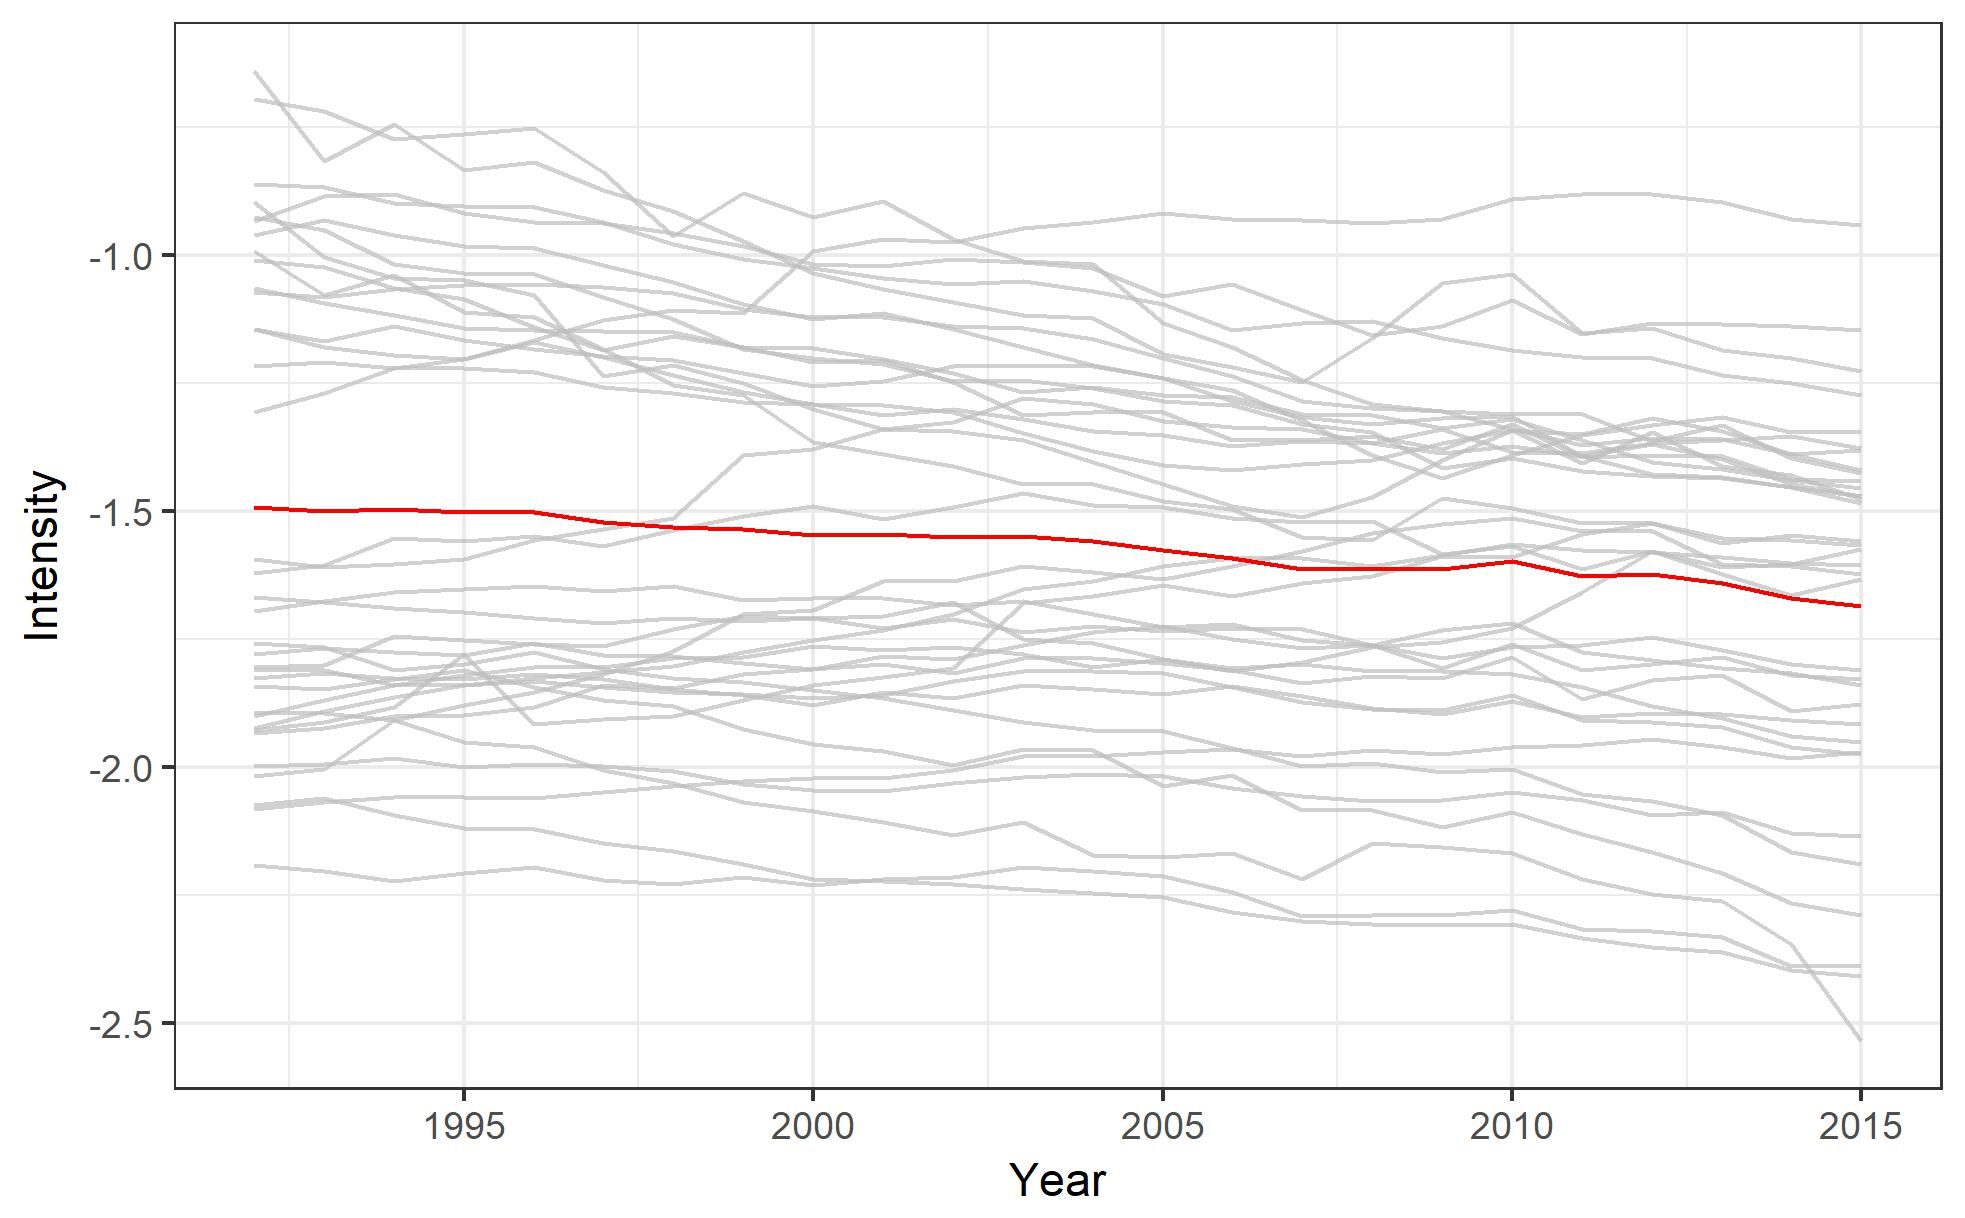
\includegraphics[height=0.5\textheight,width=1\textwidth]{Intensity_Total_trend}
    \label{Fig_levels}
\end{figure}
\newpage
\begin{figure}[ht]
  \centering
  \caption{The Variance of Total Electricity Intensity}
  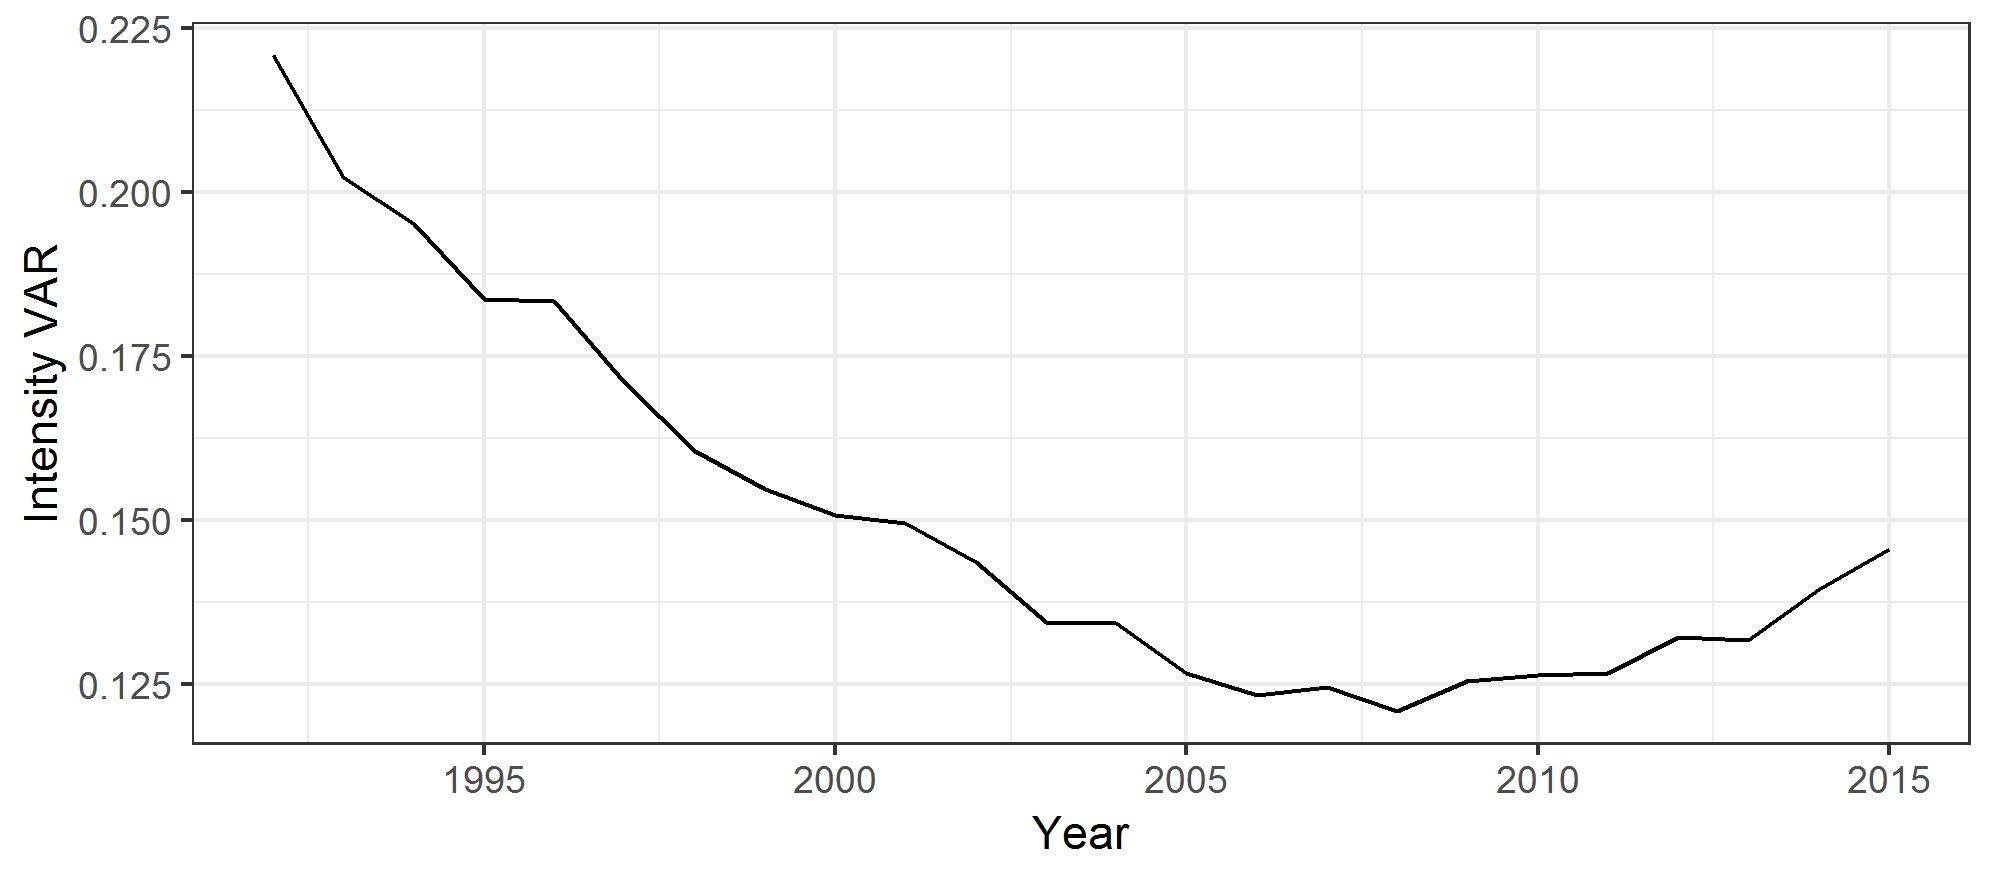
\includegraphics[height=0.4\textheight,width=1\textwidth]{OECD_Total_Filtered_VAR}
    \label{Fig_var}
\end{figure}
\bigskip
\newpage
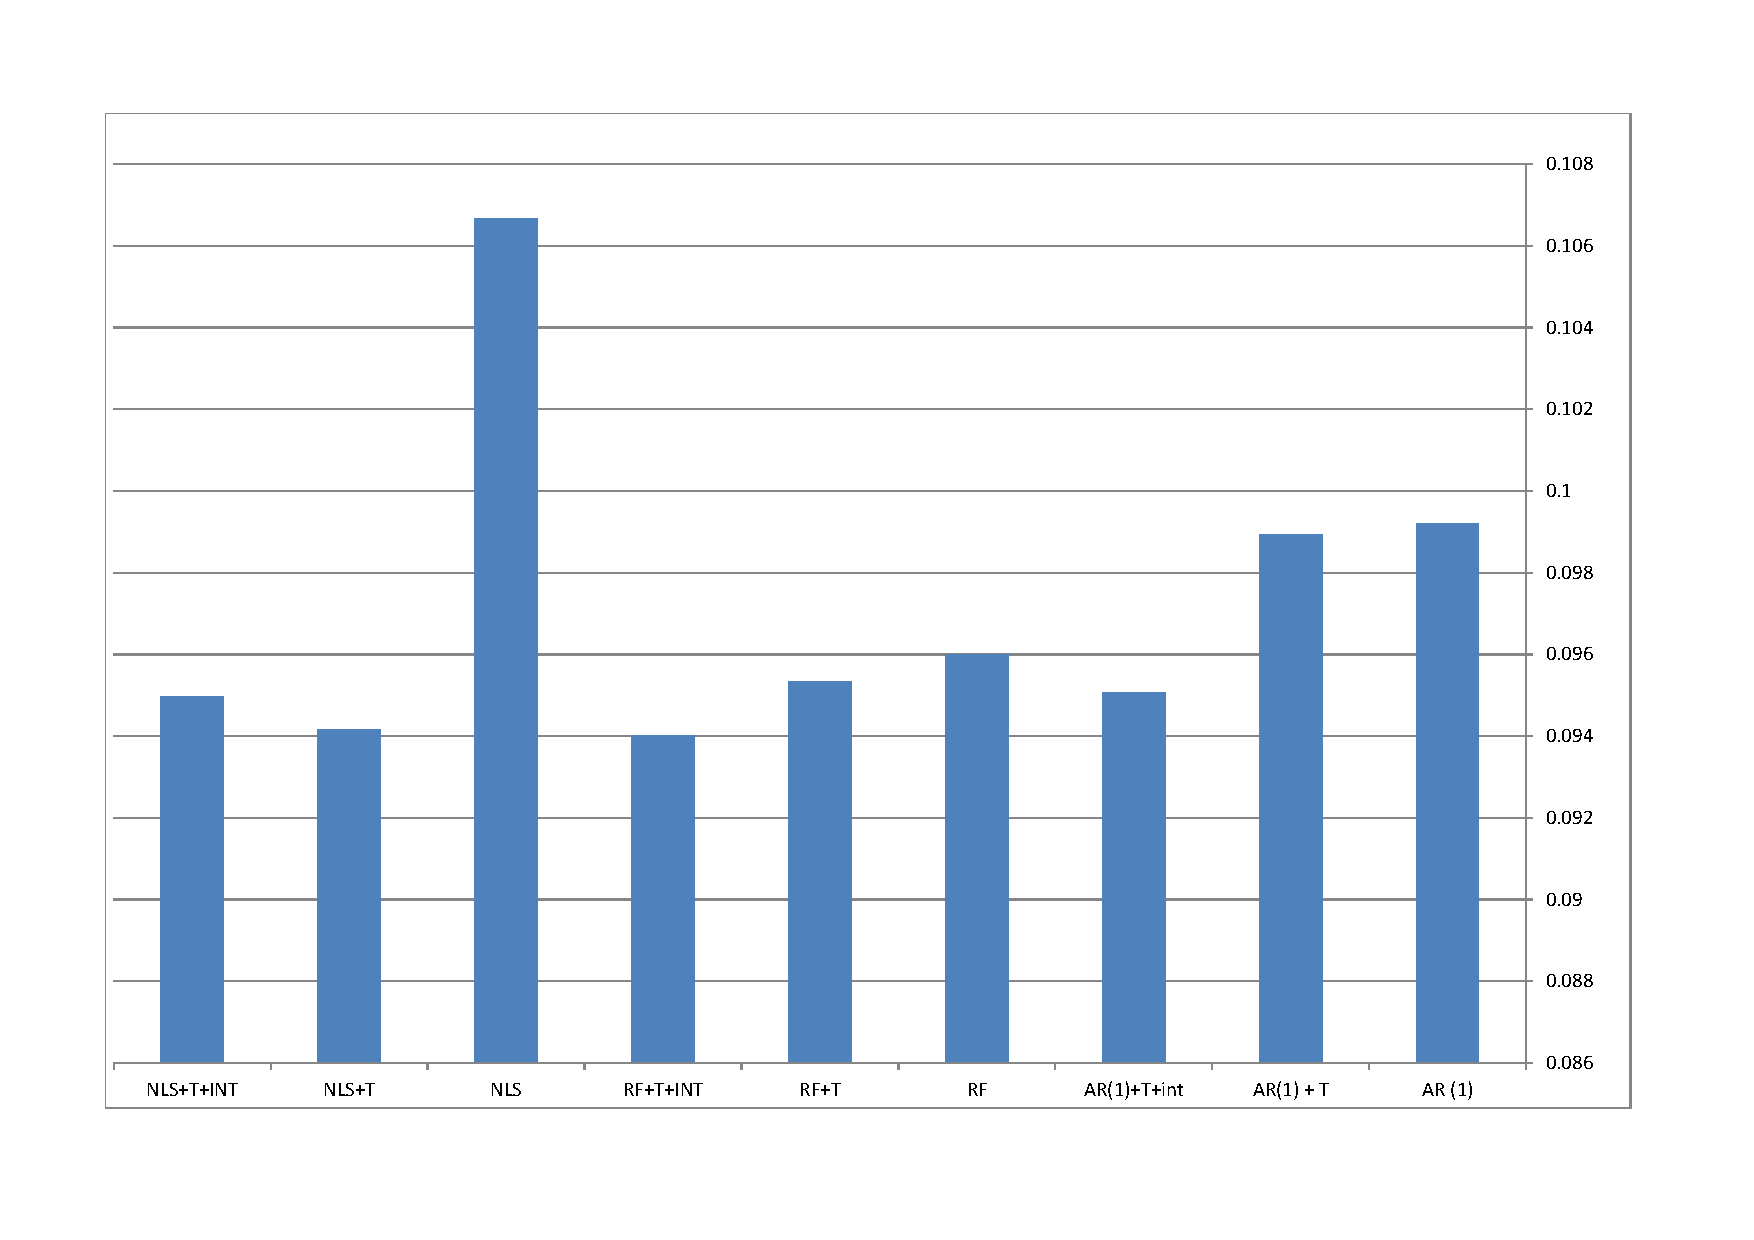
\includepdf[page=1]{Out_1.pdf}
\newpage
 


\begin{table}[htb] \centering
  \caption{$\beta$-Convergence tests: Auto-regressive, \cite{barro1992convergence} and its Reduced Form}
   \label{tbl:Beta-conv}
			\resizebox{0.7\textwidth}{!}{
			
\begin{tabular}{lccc}
    \toprule    
    \multicolumn{4}{c}{} \\
    \multicolumn{4}{c}{Panel A: Generalized Auto-regressive} \\
    \multicolumn{4}{c}{$\Delta i_{j,t} = \alpha_{AR}+ \beta_{AR} i_{j,t-1}+\gamma_{AR} t+\delta_{AR} i_{j,t-1}t+u_{j,t}$} \\
    \multicolumn{4}{c}{} \\
    \midrule

   & Model (1) & Model (2) &  Model (3)  \\ 
\hline  

{$\beta_{AR}$} & \multicolumn{1}{c}{-0.0131$^{**}$} & \multicolumn{1}{c}{-0.0143$^{**}$} &\multicolumn{1}{c}{-4.4685$^{***}$}  \\ 

  & (0.0066)& (0.0066) &  (1.0689)  \\ 

$\gamma_{AR}$ &  & \multicolumn{1}{c}{-0.0005$^{***}$}  & \multicolumn{1}{c}{-0.0124$^{***}$}  \\ 

  & & \multicolumn{1}{c}{(0.0002)} &\multicolumn{1}{c}{(0.0028)} \\ 

$\delta_{AR}$ &  &  & \multicolumn{1}{c}{0.0022$^{***}$}  \\ 

  &  &   & \multicolumn{1}{c}{(0.0005)}  \\ 

$\alpha_{AR}$ & \multicolumn{1}{c}{0.0615$^{*}$} & \multicolumn{1}{c}{1.1662$^{***}$} & \multicolumn{1}{c}{24.9153$^{***}$}  \\ 

  & \multicolumn{1}{c}{(0.0357)} & \multicolumn{1}{c}{(0.3609)} & \multicolumn{1}{c}{(5.6674)} \\ 

\hline 

Observations & \multicolumn{1}{c}{805} & \multicolumn{1}{c}{805} &  \multicolumn{1}{c}{805} \\ 

RMSE & \multicolumn{1}{c}{0.0320} & \multicolumn{1}{c}{0.0318} &  \multicolumn{1}{c}{0.0313} \\ 

R$^{2}$ & \multicolumn{1}{c}{0.0244} & \multicolumn{1}{c}{0.0368} & \multicolumn{1}{c}{0.0694} \\ 

Adjusted R$^{2}$ & \multicolumn{1}{c}{0.0232} & \multicolumn{1}{c}{0.0344} & \multicolumn{1}{c}{0.0659} \\ 
  \bottomrule
    \toprule
    \multicolumn{4}{c}{} \\    
    \multicolumn{4}{c}{Panel B: Reduced form of \cite{barro1992convergence}} \\   
    \multicolumn{4}{c}{$\frac{i_{j,t}-i_{j,t0}}{t-t_0}  = \alpha_{RF} +\beta_{RF} i_{j,t_0}+\gamma_{RF} (t-t_0) +\delta_{RF} i_{j,t_0}(t-t_0)+u_{i, t}$} \\
    \multicolumn{4}{c}{} \\

    \midrule



& Model (1) & Model (2) & Model(3)  \\ 
\hline 

$\beta_{RF}$ & \multicolumn{1}{c}{-0.0225$^{***}$} & \multicolumn{1}{c}{-0.0225$^{***}$} & \multicolumn{1}{c}{-0.0259$^{***}$}  \\ 

  & \multicolumn{1}{c}{(0.0043)} & \multicolumn{1}{c}{(0.0043)}  & \multicolumn{1}{c}{(0.0066)}  \\ 

$\gamma_{RF}$ &  & \multicolumn{1}{c}{-0.0002$^{**}$} & \multicolumn{1}{c}{-0.0016}  \\ 

  & & \multicolumn{1}{c}{(0.0001)} &\multicolumn{1}{c}{(0.0013)} \\ 
  
$\delta_{RF}$ &  &  & \multicolumn{1}{c}{0.0003}  \\ 
  &  &   & \multicolumn{1}{c}{(0.0003)}  \\ 
  
{$\alpha_{RF}$} & \multicolumn{1}{c}{0.1164$^{***}$} & \multicolumn{1}{c}{0.1192$^{***}$} & \multicolumn{1}{c}{0.1373$^{***}$}  \\
 
  & \multicolumn{1}{c}{(0.0238)} & \multicolumn{1}{c}{(0.0232)} & \multicolumn{1}{c}{(0.0349)} \\ 
\hline 

Observations & \multicolumn{1}{c}{805} & \multicolumn{1}{c}{805}  & \multicolumn{1}{c}{805} \\ 

RMSE & \multicolumn{1}{c}{0.376} & \multicolumn{1}{c}{0.383} & \multicolumn{1}{c}{0.385} \\ 

R$^{2}$ & \multicolumn{1}{c}{0.3762} & \multicolumn{1}{c}{0.3829} & \multicolumn{1}{c}{0.3851} \\ 

Adjusted R$^{2}$ & \multicolumn{1}{c}{0.375} & \multicolumn{1}{c}{0.381} & \multicolumn{1}{c}{0.383} \\ 
\bottomrule 
    \toprule
    \multicolumn{4}{c}{} \\
    \multicolumn{4}{c}{Panel C: \cite{barro1992convergence}} \\   
    \multicolumn{4}{c}{$\frac{i_{j,t}-i_{j,t0}}{t-t_0}  = \alpha_{BSM} - \left( \frac{1- e^{-\beta_{BSM}(t-t_0)}}{t-t_0} \right) i_{j,t_0}+ \gamma_{BSM}(t-t_0)+ \delta_{BSM}i_{j,t_0}(t-t_0)+u_{i, t}$} \\
    \multicolumn{4}{c}{} \\
    \midrule

 & Model (1)  & Model (2) & Model (3)\\ 
\hline 

$\alpha_{BSM}$ & \multicolumn{1}{c}{0.0624$^{***}$} & \multicolumn{1}{c}{0.137$^{***}$} & \multicolumn{1}{c}{0.132$^{***}$} \\ 
  & \multicolumn{1}{c}{(0.0142)} & \multicolumn{1}{c}{(0.0308)} & \multicolumn{1}{c}{(0.0338)}\\ 

$\beta_{BSM}$ & \multicolumn{1}{c}{0.0137$^{***}$} & \multicolumn{1}{c}{0.0261$^{***}$} & \multicolumn{1}{c}{0.0251$^{***}$} \\ 

  & \multicolumn{1}{c}{(0.00316)} & \multicolumn{1}{c}{(0.00591)} & \multicolumn{1}{c}{(0.00659)} \\ 
$\gamma_{BSM}$ &  & \multicolumn{1}{c}{-0.00169$^{***}$}& \multicolumn{1}{c}{-0.00127} \\ 
  &  & \multicolumn{1}{c}{(0.000561)} & \multicolumn{1}{c}{(0.00125)} \\ 
$\delta_{BSM}$ &  &  & \multicolumn{1}{c}{-0.0000} \\ 
  &  &  &\multicolumn{1}{c}{(0.000163)}\\ 

\hline

Observations & \multicolumn{1}{c}{805} & \multicolumn{1}{c}{805} & \multicolumn{1}{c}{805} \\ 

RMSE & \multicolumn{1}{c}{0.0148} & \multicolumn{1}{c}{0.0134} & \multicolumn{1}{c}{0.0134} \\ 

R$^{2}$ & \multicolumn{1}{c}{0.243} & \multicolumn{1}{c}{0.383} & \multicolumn{1}{c}{0.383}\\ 

Adjusted R$^{2}$ & \multicolumn{1}{c}{0.221} & \multicolumn{1}{c}{0.365} & \multicolumn{1}{c}{0.365} \\ 
\bottomrule
  \multicolumn{1}{l}{Note:\ $^{*}$p$<$0.1; $^{**}$p$<$0.05; $^{***}$p$<$0.01 \endgraf}

  \end{tabular}
}
\end{table}


\newpage

	\begin{table}[htb]
		\caption{$\sigma$ Test for the Convergence of Electricity Intensity}
		\label{tbl:Sigma_Results}

		\begin{center}
			\begin{tabular}{lcc}
				\toprule    
				\multicolumn{3}{c}{} \\
				\multicolumn{3}{c}{Panel A: \cite{PhillipsSul2007}} \\
				\multicolumn{3}{c}{$\log{ \left( \frac{\hat \sigma_1^2}{\hat \sigma_t^2} \right)} - 2\log{ \log{(t+1)}} = \alpha_{PS} + \beta_{PS} \log{(t)}+\gamma_{PS} \log{(t)}^2+\epsilon_{j,t}$} \\
				\multicolumn{3}{c}{} \\
				\midrule
				
				& Model (1) & Model (2)  \\ 
				\hline 
				
				$\beta_{PS}$ & \multicolumn{1}{c}{37.317$^{***}$} & \multicolumn{1}{c}{133835.8$^{***}$}   \\ 
				
				& (5.949)& (9523.5)  \\ 
				
				$\gamma_{PS}$ &  & \multicolumn{1}{c}{-8799.2$^{***}$}    \\ 
				
				& & \multicolumn{1}{c}{(626.3)}  \\ 
				
				{$\alpha$} & \multicolumn{1}{c}{-287.359$^{***}$} & \multicolumn{1}{c}{-508914.8$^{***}$}   \\ 
				
				& \multicolumn{1}{c}{(45.228)} & \multicolumn{1}{c}{(36202.9)} \\ 
				
				\hline  
				
				Observations & \multicolumn{1}{c}{23} & \multicolumn{1}{c}{23} \\ 
				
				RMSE & \multicolumn{1}{c}{0.09} & \multicolumn{1}{c}{0.027}  \\ 
				
				R$^{2}$ & \multicolumn{1}{c}{0.652} & \multicolumn{1}{c}{0.968} \\ 
				
				Adjusted R$^{2}$ & \multicolumn{1}{c}{0.636} & \multicolumn{1}{c}{0.965}  \\ 
				\bottomrule
				\toprule    
				\multicolumn{3}{c}{} \\
				\multicolumn{3}{c}{Panel B: AR(1) model of variance} \\
				\multicolumn{3}{c}{$Var_{t}(u_{i,t})= Var_{t}(i_{j,t}) + (1-\beta)^2Var_{t-1}(i_{j,t-1})$} \\
				\multicolumn{3}{c}{} \\
				\midrule
					
					& Model (1) & Model (2)  \\ 
					\hline 
					{$(1-\beta)^2$} & \multicolumn{1}{c}{0.973$^{***}$} & \multicolumn{1}{c}{0.8332$^{***}$}   \\ 
					
					
					& (0.008)& (0.0337)  \\ 
					
					{Constant} &  & \multicolumn{1}{c}{0.0218$^{***}$}   \\ 
					
					& & \multicolumn{1}{c}{(0.0337)} \\ 
					
					\hline 
					
					Observations & \multicolumn{1}{c}{23} & \multicolumn{1}{c}{23} \\ 
					
					RMSE & \multicolumn{1}{c}{0.006} & \multicolumn{1}{c}{0.004}  \\ 
					
					R$^{2}$ & \multicolumn{1}{c}{0.998} & \multicolumn{1}{c}{0.967} \\ 
					
					Adjusted R$^{2}$ & \multicolumn{1}{c}{0.998} & \multicolumn{1}{c}{0.965}  \\ 
					\bottomrule
					\multicolumn{3}{l}{Note:\ $^{*}$p$<$0.1; $^{**}$p$<$0.05; $^{***}$p$<$0.01 \endgraf}
				\end{tabular}
			\end{center}
			

		\end{table}


%%%%%%%%%%%%%%%%%%%%%%%%%%%%%%% Appendices %%%%%%%%%%%%%%%%%%%%%%%%%%%%%%%%%%%%

\setcounter{table}{0} \renewcommand{\thetable}{B\arabic{table}}
\begin{appendices}


\section{Data Appendix}
  
  
    \thispagestyle{empty}
		\begin{table}[] \centering 
			\resizebox{1\textwidth}{!}{
	  		\label{table_OBS}
	  		 
\begin{tabular}{@{\extracolsep{5pt}}lD{.}{.}{-3} D{.}{.}{-3} D{.}{.}{-3} D{.}{.}{-3} D{.}{.}{-3} D{.}{.}{-3} D{.}{.}{-3} } 
\\[-1.8ex]\hline 
\hline \\[-1.8ex] 
 & \multicolumn{7}{c}{Final Database Observation Summery } \\ 
\cline{2-8} 
 & \multicolumn{1}{c}{Total} & \multicolumn{1}{c}{Households} & \multicolumn{1}{c}{Agriculture} & \multicolumn{1}{c}{Mining} & \multicolumn{1}{c}{Manufacturing} & \multicolumn{1}{c}{Construction} & \multicolumn{1}{c}{Services} \\ 

\hline \\[-1.8ex] 
Countries & \multicolumn{1}{c}{35} & \multicolumn{1}{c}{36} & \multicolumn{1}{c}{32} & \multicolumn{1}{c}{28} & \multicolumn{1}{c}{35} & \multicolumn{1}{c}{24} & \multicolumn{1}{c}{34} \\ 
Years & \multicolumn{1}{c}{24} & \multicolumn{1}{c}{24} & \multicolumn{1}{c}{24} & \multicolumn{1}{c}{23} & \multicolumn{1}{c}{24} & \multicolumn{1}{c}{24} & \multicolumn{1}{c}{24} \\ 
Observations & \multicolumn{1}{c}{840} & \multicolumn{1}{c}{864} & \multicolumn{1}{c}{768} & \multicolumn{1}{c}{644} & \multicolumn{1}{c}{840} & \multicolumn{1}{c}{576} & \multicolumn{1}{c}{816} \\ 

\hline 
\hline \\[-1.8ex] 
\\ 
\end{tabular}  
}
		\end{table} 
  
In order to conduct this analysis, we collected data and created a balanced panel dataset for the following countries(36):
Australia, Austria, Belgium, Canada, Chile, Czech Republic, Denmark, Estonia, Finland, France, Germany, Greece, Hungary, Iceland, Ireland, Israel, Italy, Japan, Latvia, Lithuania, Luxembourg, Mexico, Netherlands, New Zealand, Norway, Poland, Portugal, Republic of Korea, Slovakia, Slovenia, Spain, Sweden, Switzerland, Turkey, United Kingdom and United States.

For each of the following countries we collected data on six branches of economy: Agriculture, Mining and Querying, Manufacturing, Commercial
Services and Construction. In addition to consumption by Households and Gross Consumption.

A list of the data collected:

\begin{enumerate}
  \item Electricity consumption and its breakdown by sectors in million Kilowatts per hours, as published by the UNSTATS. Covering 1990-2016.
  \item GDP and its breakdown at constant 2010 prices in US Dollars, as published by the UNSTATS National accounts main aggregates database. Covering 1970-2016.
  \item Per capita GDP at current prices – US dollars as published by the UN statistics division. Covering 1970-2016.
\end{enumerate}
		\subsubsection{Sources Limitations}
		our dataset is limited in several aspects:
		 \begin{enumerate}
  \item UNSTATS breakdown to sectors of electricity consumption was not paralleled to UNSTATS breakdown to sectors of states GDP (ISIC Rev. 4). therefore we used the UNSTATS "guidelines for the 2016 united nations statistics division annual questionnaire on energy statistics" in order to correspond to ISIC Rev. 4.
  \begin{description}
  \item[$\bullet$ Total] "Final energy consumption" (CL12)
  \item[$\bullet$ Mining] "Mining and quarrying" (CL1214e)
  \item[$\bullet$ Construction] "construction" (CL1214i)
  \item[$\bullet$ Households] "Households" (CL1231)
  \item[$\bullet$ Agriculture] "Agriculture, forestry and fishing" (CL1232)
  \item[$\bullet$ Services] "Commerce and public services" (CL1235)
  \item[$\bullet$ Manufacturing] We took the "Manufacturing, Construction, and non-fuel mining industry" (CL121) and reduced the mining (CL1214e) and Construction (CL1214i) industries. 
  
  \end{description}
  \item in order to have a balanced panel dataset for each sector, we had to make sure we have continuous series for each country in each sector. due to this reason we had to remove from our dataset the following states in the following sectors: 
  	\begin{enumerate} 
  	\item In the Agriculture industries we removed the following counties:
		\begin{enumerate}   	 
  	  	\item Belgium, due to lack of data for 1990-1996
  	  	\item Germany, no data at all
  	  	\item Slovenia, no data at all
  	  	\item United States, due to lack of data for 1990-2001
  		\end{enumerate}
  	\item In the Commercial Services industries we removed the following counties:
		\begin{enumerate}   	 
  	  	\item Latvia, due to lack of data for 1998-2006
  	  	\item Lithuania, due to lack of data for 1990-2006
  		\end{enumerate}
  	\item In the construction industry we removed the following counties:
		\begin{enumerate}   	 
  	  	\item Slovenia, due to lack of data for 1997-1999
        \item Canada, No data at all
        \item Chile, No data at all
        \item Germany, due to lack of data for 2003-2015
        \item Greece, due to lack of data for 2015
        \item Israel, due to lack of data for 2013-2015
        \item Latvia, due to lack of data for 1990-2006
        \item Lithuania, due to lack of data for 1990-2006
        \item Luxembourg, due to lack of data for 1990-1999
        \item Republic of Korea, No data at all                 
        \item Slovakia, due to lack of data for 1992
        \item United States, due to lack of data for 1990-2002
 		\end{enumerate}
	\item In the Mining industries we removed the following counties:
		\begin{enumerate}   	 
        \item Latvia, due to lack of data for 1990-2006
        \item Lithuania, due to lack of data for 1990-2006
        \item Luxembourg, due to lack of data for 1990-1999
        \item Slovakia, due to lack of data for 1990-1994
        \item Slovenia, due to lack of data for 1990-1996
        \item Sweden, missing data for 2014
        \item Switzerland, no data at all
        \item United Kingdom, due to lack of data for 1990-2009
  		\end{enumerate}
  	\item Iceland was removed from both the Manufacturing industries and the Total groups, due to dramatic chances in the Icelandic economy, further discussion on the Icelandic case will be follow.
  	\end{enumerate}
\end{enumerate}

\newpage

\bibliographystyle{plainnat}
\bibliography{OECD}

\newpage
\setcounter{table}{0} \renewcommand{\thetable}{B\arabic{table}}

	\end{appendices}
 \end{document}